\documentclass[article,12pt,onesidea,4paper,english,brazil]{abntex2}

\usepackage{lmodern, indentfirst, nomencl, color, graphicx, microtype, lipsum, textcomp, newfloat}			
\usepackage[T1]{fontenc}		
\usepackage[utf8]{inputenc}		

\setlrmarginsandblock{2cm}{2cm}{*}
\setulmarginsandblock{2cm}{2cm}{*}
\checkandfixthelayout

\setlength{\parindent}{1.3cm}
\setlength{\parskip}{0.2cm}

\SingleSpacing

\DeclareFloatingEnvironment[fileext=qud,listname={Lista de Quadros},placement={!ht},name=Quadro]{quadro}

\begin{document}

	\selectlanguage{brazil}
	
	\frenchspacing 
	
	\begin{center}
		\LARGE 
		AVALIAÇÃO DE APARELHO GPS NAVEGAÇÃO GARMIN ETREX 20 EM RELAÇÃO À MEDIÇÃO DE ÁREA NO CENTRO UNIVERSITARIO LUTERANO DE JI-PARANÁ – CEULJI/ULBRA – RO
		
		\normalsize
		Dayane Rodrigues Raasch\footnote{Discente do curso técnico em florestas – IFRO. e-mail: dayane.raasch@gmail.com} 
		Selma Maria de Arruda Silva2\footnote{Professora de Geografia - IFRO. e-mail: selma.arruda@ifro.edu.br} 
	 
	\end{center}
	
	% resumo em português
	\begin{resumoumacoluna}
O sistema de navegação GPS é uma das tecnologias mais usadas atualmente, seja para deslocamento, localização e demarcação de coordenadas e áreas, passeios e aviação entre outros. O objetivo deste trabalho é avaliar a confiabilidade do aparelho GPS de navegação na obtenção de dados para mapeamento e determinação de uma área de um terreno. Para esta avaliação foram realizadas três medições em dias alternados.
		
		\vspace{\onelineskip}
		
		\noindent
		\textbf{Palavras-chave}: Levantamento De Área. Cartografia. Geotecnologia.
	\end{resumoumacoluna}
	
	\textual
	
	\section*{Introdução}
	
	Nos dias atuais, é cada vez mais frequente o uso de tecnologia do Sistema de Posicionamento Global (GPS) para medição e mapeamento de áreas urbanas e rurais. Projetado e desenvolvido por agências americanas, sendo baseado em satélites. Originalmente foi criado para uso militar e posteriormente disponibilizado para o uso civil em 2000, pelo Presidente Bill Clinton.
	
	\section*{Material e Método}
	
O experimento foi realizado no campo experimental do Centro Universitário Luterano de Ji-Paraná (CEULJI/ULBRA) localizado no município de Ji-Paraná-RO com a coordenada geográfica pelo paralelo de latitude 10º 51’ 40,32” S em sua intersecção com o meridiano de longitude 61º 57’ 34,56” W, estando a uma altitude de 175 metros conforme Figura 1.

Para realização do presente estudo foi utilizado um aparelho GPS de navegação Garmin Etrex 20 e demais matérias de auxilio no levantamento.

Foram realizadas medições em dias alternados com o auxílio do GPS navegação com os tempos de 0 e 5 minutos com três repetições realizadas nos dias 18, 19 e 28 de maio de 2015 sempre no mesmo horário as 15:00 h.

	\begin{figure}[h]
	\centering
	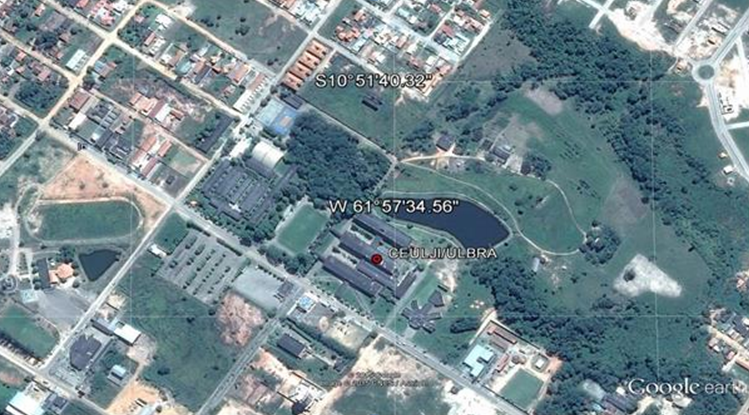
\includegraphics[width=0.7\linewidth]{pip05.png}
	\caption{Imagem do Centro Universitário Luterano de Ji-Paraná.}
\end{figure}

Depois de realizados os levantamentos de campo, os dados coletados com aparelho GPS foram descarregados em um microcomputador com auxílio do programa GPS TRACKMAKER usado na elaboração do mapeamento das áreas e processamento dos dados gravados conforme tabelas abaixo.

\begin{quadro}[h]
	\centering
	\caption{Coordenadas levantadas a campo com o tempo de 0 minuto de estabilização e gravação}
	\label{my-label}
	\begin{tabular}{c|c|c|c|c|c|c|}
		\cline{2-7}
		& \multicolumn{6}{c|}{DATAS DE LEVANTAMENTOS COORDENADAS UTM}                                         \\ \cline{2-7} 
		& \multicolumn{2}{c|}{18/05/2015} & \multicolumn{2}{c|}{19/05/2015} & \multicolumn{2}{c|}{28/05/2015} \\ \hline
		\multicolumn{1}{|c|}{PONTOS} & ESTE           & NORTE          & ESTE           & NORTE          & ESTE           & NORTE          \\ \hline
		\multicolumn{1}{|c|}{1}      & 613795,573     & 8799016,916    & 613798,091     & 8799018,013    & 613794,696     & 8799016,255    \\ \hline
		\multicolumn{1}{|c|}{2}      & 613837,319     & 8799013,566    & 613838,199     & 8799015,221    & 613834,372     & 8799014,903    \\ \hline
		\multicolumn{1}{|c|}{3}      & 613871,851     & 8799074,492    & 613870,540     & 8799074,717    & 613871,531     & 8799076,594    \\ \hline
		\multicolumn{1}{|c|}{4}      & 613942,433     & 8799160,287    & 613943,094     & 8799161,612    & 613940,354     & 8799159,631    \\ \hline
		\multicolumn{1}{|c|}{5}      & 613934,251     & 8799165,070    & 613932,838     & 8799167,287    & 613930,093     & 8799163,647    \\ \hline
		\multicolumn{1}{|c|}{6}      & 613865,323     & 8799147,060    & 613866,425     & 8799149,821    & 613861,065     & 8799148,623    \\ \hline
		\multicolumn{1}{|c|}{7}      & 613821,993     & 8799102,973    & 613822,110     & 8799105,295    & 613819,918     & 8799103,422    \\ \hline
	\end{tabular}
\end{quadro}

\begin{quadro}[!h]
	\centering
	\caption{Coordenadas levantadas a campo com o tempo de 5 minutos de estabilização e gravação.}
	\label{my-label}
	\begin{tabular}{|c|c|c|c|c|c|c|}
		\hline
		\multicolumn{7}{|c|}{DATAS DE LEVANTAMENTOS COORDENADAS UTM}                                                 \\ \hline
		& \multicolumn{2}{c|}{18/05/2015} & \multicolumn{2}{c|}{19/05/2015} & \multicolumn{2}{c|}{28/05/2015} \\ \hline
		PONTOS & ESTE           & NORTE          & ESTE           & NORTE          & ESTE           & NORTE          \\ \hline
		1      & 613797,104     & 8799017,131    & 613796,122     & 8799017,798    & 613794,364     & 8799015,150    \\ \hline
		2      & 613837,319     & 8799013,676    & 613837,651     & 8799014,891    & 613836,334     & 8799013,237    \\ \hline
		3      & 613871,969     & 8799076,924    & 613873,608     & 8799076,808    & 613869,243     & 8799078,924    \\ \hline
		4      & 613942,984     & 8799161,391    & 613942,003     & 8799162,169    & 613936,531     & 8799160,307    \\ \hline
		5      & 613932,720     & 8799164,744    & 613932,504     & 8799165,519    & 613928,788     & 8799165,753    \\ \hline
		6      & 613866,089     & 8799147,389    & 613866,098     & 8799150,043    & 613862,704     & 8799148,396    \\ \hline
		7      & 613824,404     & 8799104,624    & 613822,660     & 8799106,178    & 613820,034     & 8799105,413    \\ \hline
	\end{tabular}
\end{quadro}

O cálculo da área foi realizado através de planilha eletrônica Excel com a formulação das células baseadas na fórmula do cálculo de áreas de GAUSS, utilizando as coordenadas limites de cada área.

	
	\section*{Resultados e Discussão}
	
	O primeiro ponto demarcado com o GPS localizado no Centro Universitário Luterano de Ji-Paraná.
	Os resultados dos levantamentos efetuados se encontram nos quadros 3 e 4. 
	
	\begin{quadro}[h]
		\centering
		\caption{Dados processados para o levantamento a campo com o tempo de 0 minuto de estabilização e gravação.}
		\label{my-label}
		\footnotesize
		\begin{tabular}{|c|c|c|c|c|c|}
			\hline
			DATA                                                              & PERIMETRO (m)         & ÁREA (m²)             & ÁREA (ha) DIFERENÇA   & (ha) DIFERENÇA        & (m²)                  \\ \hline
			18.05.2015	                                                    & 455,57                & 8.646,7365            & 0,8647                & -                     & -                     \\ \hline
			\begin{tabular}[c]{@{}c@{}}18.05.2015 a\\ 19.05.2015\end{tabular} & 454,87                & 8656,1169             & 0,8656                & 0,0009                & 9                     \\ \hline
			\begin{tabular}[c]{@{}c@{}}19.05.2015 a\\ 2.05.2015\end{tabular}  & 453,10                & 8.684,0215            & 0,8684                & 0,0028                & 28                    \\ \hline
		\end{tabular}
	\end{quadro}
	
	No Quadro 3 o resultado que apresentou maior diferença encontrada nos levantamentos a campo foi entre os dia 19.05.2015 e o dia 28.05.2015 com 28 m².
	
	\begin{quadro}[h]
		\centering
		\caption{Dados processados para o levantamento a campo com o tempo de 5 minutos de estabilização e gravação.}
		\label{my-label}
		\footnotesize
		\begin{tabular}{|c|c|c|c|c|c|}
			 \hline
			DADOS                                                             & PERIMETRO (m) & ÁREA (m²)  & ÁREA (ha) DIFERENÇA & (ha) DIFERENÇA & (m²)  \\ \hline
			18.05.2015                                                        & 453,86        & 8.336,0619 & 0,8336              & -              & -     \\ \hline
			\begin{tabular}[c]{@{}l@{}}18.05.2015 a\\ 19.05.2015\end{tabular} & 454,88        & 8.744,0635 & 0,8744              & 0,0408         & 408   \\ \hline
			\begin{tabular}[c]{@{}l@{}}19.05.2015 a\\ 28.05.2015\end{tabular} & 452,44        & 8.401,7102 & 0,8402              & -0,0342        & -342  \\ \hline
		
		\end{tabular}
	\end{quadro}

No Quadro 4 o resultado que apresentou maior diferença encontrada nos levantamentos a campo foi entre os dia 18.05.2015 e o dia 19.05.2015 com 408 m².
Após avaliação, os resultados demonstraram que existe diferença na localização espacial dos pontos coletados com o aparelho GPS. Esta variação resulta numa diferença na sobreposição dos mapas gerados nas três coletas, bem como gera aumento ou decréscimo nos valores das áreas calculadas.

	
	\section*{Conclusões}
	
	Os melhores resultados encontrados neste trabalho com o uso de sistema de posicionamento global – GPS foram para o levantamento em tempo real, 0 minutos, sendo a diferença maior encontrada nos três dias de levantamento de 28 m².
	
	\section*{Instituição de Fomento}
	
	Instituto Federal de Ciência e Tecnologia- IFRO / Campus Ji-Paraná, forneceu os tipos de GPS para a realização da pesquisa.
	
	\sloppy
	\section*{Referências}
	
	\noindent BORGES, A. C. Topografia aplicada a Engenharia. 3. Ed. São Paulo, Blucher, 2013.GOMES, E.; PESSOA, L. M. C.; JÚNIOR, L. B. S. Medindo Imóveis Rurais
	com GPS. Brasília, LK-Editora, 2001, p. 136.
	
	
	\noindent Normas e padrões para trabalhos acadêmicos e científicos da unoeste. Universidade do Oeste Paulista – UNOESTE, Presidente Prudente, São Paulo. Disponivel em: <https://unoeste.br/site/biblioteca/documentos/Manual-Normalizacao.pdf>  Acesso em: 03 de agosto de2015.
	
	\noindent ROCHA, C. H. B. Geoprocessamento – Tecnologia Transdisciplinar. Minas Gerais, Ed. do Autor, 2000, 220p.
	
	\noindent ZANOTTA, D. C; CAPELLETTO, E; MATSUOKA. O GPS: unindo ciência e
	tecnologia em aulas de física. Revista Brasileira de Ensino de Física, v. 33, n. 2, 2313 (2011). Disponível em: <http://www.scielo.br/scielo.php?pid=S1806-11172011000200014\&script=sci\_arttext> . Acesso em: 06 de agosto 2015.

\end{document}